\section{Numerical Experiments}

\subsection{Travelling Wave Allen Cahn}
In this section we run numerical experiments compairing the backward Euler method to krylov methods for computing solutions to a PDE.
Specifically we will investigate the initial boundary value problem for the Allen Cahn equation on a strip with a traveling wave solution\cite{YukitakaFukao2004} given by:

\begin{align}
    \hat u(x,y,t)&=\frac{e^{\frac{x-ct}{\sqrt2}}}{1+e^{\frac{x-ct}{\sqrt2}}} \label{TravelingWaveSol}\\
    \text{where } c &= \frac{\sqrt{2}}{4}
\end{align}
and where the problem is defined as follows:
\begin{align*}
    u_t&=\Delta u+u(u-\frac14)(1-u) \text{ on $\Omega \times [0, 8]$}\\
    \text{with } \Omega &= \mathbb{R}\times[-1,1]\\
    \nabla u \cdot \hat n &= g \text{ for $g = \nabla \hat u \cdot \hat n$}\\
    u_0(x, y) &= \hat u(x,y, 0)\\
\end{align*}
However for our numerical experiments we compute on the space $\Omega=[-16,16]\times[-1,1]$.
Where $u$ is the solution, we write it in weak form.
\begin{align*}
    \dot u&=\Delta u+u(u-\frac14)(1-u)\\
    \int_{\Omega} \dot u v &=\int_{\Omega} \Delta uv+u(u-\frac14)(1-u)v \text{ for a smooth function $v \in C^{\infty}(\overline{\Omega})$}\\
    \int_{\Omega} \dot u v &=\int_{\Omega} u(u-\frac14)(1-u)v - \nabla u \cdot \nabla v + \int_{\partial\Omega}  v\hat n \cdot \nabla u\\
    \text{subsituting in } u_h(t,x,y) &= \sum_i u_i(t) v_i(x,y) \text{ where $(v_i)$ are the test functions we obtain:}\\
    \text{we get } \sum_i\int_{\Omega} \dot u_i v_i v_j &=\sum_i(\int_{\Omega} u_iv_i(u_iv_i-\frac14)(1-u_iv_i)v_j - \int_{\Omega}\nabla (u_iv_i) \cdot \nabla v_j + \int_{\partial\Omega}  v_j\hat n \cdot \nabla \hat u_iv_i)\\
    \sum_iu_i\int_{\Omega}v_iv_j &= -u_i\sum_i(\int_{\Omega}\nabla v_i \cdot \nabla v_j + \int_{\Omega}R(u_h)v_j)\\
    \text{where we have } R(u)&=u(u-\frac14)(1-u) + \int_{\partial\Omega}  \hat n \cdot \nabla \hat  u\\
    \intertext{The above is true for all $i=0,1,2,...,n$. Writing in matrix vector form gives}
    M \underline{\dot u} &= DN(\underline{u})\underline{u} + R(\underline{u})\\
    \text{where } M_{i,j} &= \int_{\Omega}v_iv_jdx
\end{align*}
In the tests, we will investigate the relation between step size, $L_2$ error given by $||\hat u - \underline{u}||_{L_2}$ and call to the operator $N$ which will be a crude approximation to the computational cost.
We compare the Backward Euler, First and Second order expoenntial methods over grid sizes: $128 \times 8$ and $256 \times 8$ and with time step $\tau=8,4,2,1,0.5,0.25,0.125,0.0625,0.03125$.

\subsubsection{Experimental Results}

Bellow we show the $L_2$ error with respect to the time step $\tau$.
Where in the legend EXP1LAN 16 denotes the first order method with Krylov size 16, likewise for EXP2LAN and the second order method.
BE denotes the backwards Euler method.

\begin{figure}[H]
    \centering
    \begin{minipage}{0.49\textwidth}
        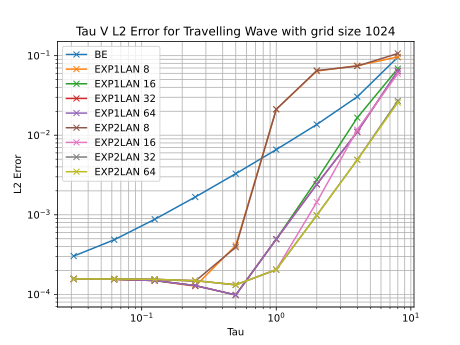
\includegraphics[width=1\textwidth]{Graphs/TravellingWave/Tau V L2 Error for Travelling Wave with grid size 1024.png} % Change filename to your image
        \caption{$\tau$ vs $L_2$ with grid size 1024}
        \label{fig:plot1}
    \end{minipage}\hfill
    \centering
    \begin{minipage}{0.49\textwidth}
        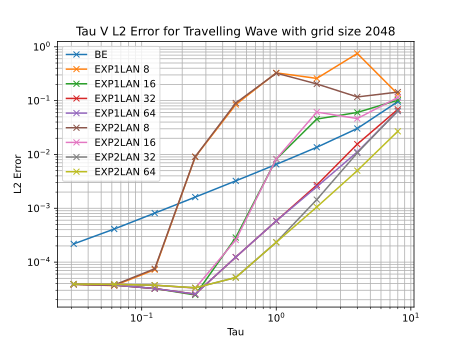
\includegraphics[width=1\textwidth]{Graphs/TravellingWave/Tau V L2 Error for Travelling Wave with grid size 2048.png} % Change filename to your image
        \caption{$\tau$ vs $L_2$ with grid size 2048}
        \label{fig:plot2}
    \end{minipage}\hfill
\end{figure}

First see that all of the methods tested converge, tending towards the discritisation error.
The discritisation error is smaller on the more detailed grid.
The Krylov methods converge faster than the backwards Euler method.
We notice that when a smaller Krylov subspace is used that the expoenntial methods only start to converge for a sufficiently small tau.
Likewise when these methods start to converge we observe that the perform simillarly to the methods using a larger subspace, however they will require fewer operator calls.
This suggests that for sufficient small time steps a shallower subspace may suffice.
Likewise for the converse that larger timesteps require a deeper krylov subspace.

Now we compare the error with the number of calls to the operator.
These operator calls are needed for computing $N$ which is used with the matrix free methods as described above as well as for computing the non-linear term $R$.

\begin{figure}[H]
    \centering
    \begin{minipage}{0.49\textwidth}
        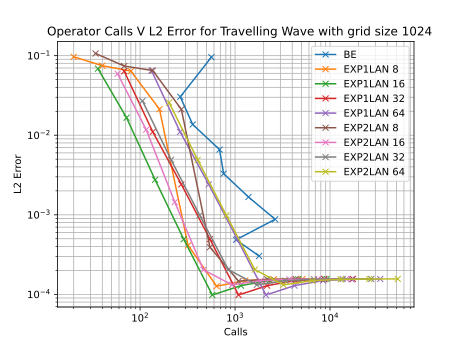
\includegraphics[width=1\textwidth]{Graphs/TravellingWave/Operator Calls V Error for Travelling Wave with grid size 1024.png} % Change filename to your image
        \caption{$\tau$ vs $L_2$ with grid size 1024}
        \label{fig:plot1}
    \end{minipage}\hfill
    \centering
    \begin{minipage}{0.49\textwidth}
        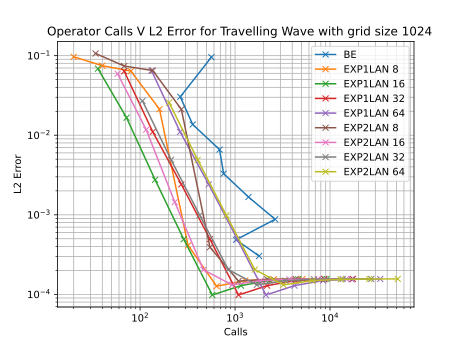
\includegraphics[width=1\textwidth]{Graphs/TravellingWave/Operator Calls V Error for Travelling Wave with grid size 1024.png} % Change filename to your image
        \caption{$\tau$ vs $L_2$ with grid size 2048}
        \label{fig:plot2}
    \end{minipage}\hfill
\end{figure}

We see that as expected that when are larger krylov subspace is used that more calls to the operator are required.
We also observe that the exponential methods outperform the BE by achieving a lower error with fewer calls to the operator.

Here we present the experimental orders of convergence.

\begin{table}[H]
    \centering
    \begin{tabular}{| c | c | c | c}
    \hline
    BE & EXP1LAN 64 & EXP2LAN 64 \\
    \hline
    1.656175178817219 & 2.5200121901844423 & 2.427488988868435 \\
    1.159963039219372 & 2.147211103525317 & 2.2448741639287576 \\
    1.0543798412512431 & 2.1084233436748687 & 2.175268892119002 \\
    1.0188791686457326 & 2.235535140373336 & 2.176237872787299 \\
    1.0016513655730614 & 2.2847781778148475 & 0.6355415381730404 \\
    0.9874831778164389 & -0.3463812590562603 & -0.1610890501147955 \\
    0.9808216274859436 & -0.2097197508087928 & -0.0545528584432596 \\
    0.919336864575657 & -0.051644372942987 & -0.01407844052927163 \\
    \hline
    \end{tabular}
    \caption{Experimental orders of convergence}
    \label{tab:EOCs}
\end{table}


We observe that the rate of convergence for the second order method was inline with what has been shown analytic\cite{Huang2022} at a rate of $2$.
The first order method converges with a rate of 2 despite an expectation of a rate of $1$\cite{Huang2022}.
The exponential methods stop converging as they reach the discritisation error.
The backwards euler converges at the rate expceted of 1.

\subsection{A 2D Allen Cahn Problem}

We will now look into the two dimentional Allen Cahn Problem given by:
\begin{align*}
    u_t &= -\Delta u + u (u^2-1) \text{ } \Omega=[0,1]\times[0,1]
\end{align*}
With Neumann boundary conditions.
The initial condition is chosen by randomly setting points on the grid from a uniform distribution in the range $-0.9,0.9$.
The same randomly generated initial condition will be used for each test.
As we do not have an exact solution, we will use the backwards Euler method with a timestep of $\tau = 10^{-4}$ to genarate a referance solution.
We will compare the backwards Euler method to the first and second order expoenntial integrator methods described above.
The tests are run on a $60\times60$ grid with the end time being $t_e=24$.
The error is computed by calculating the $L_2$ error between the prediction of the chosen stepper and the reference solution. 
Below we present our results.

\subsubsection{Experimental Results}

We begin by compairing the timestep size $\tau$ to the $L_2$ error for the different methods.

\begin{figure}[H]
    \centering
    \begin{minipage}{0.49\textwidth}
        \includegraphics[width=1\textwidth]{example-image-a} % Change filename to your image
        \caption{$\tau$ vs $L_2$ with grid size 2048}
        \label{fig:ACtauE}
    \end{minipage}\hfill
    \centering
    \begin{minipage}{0.49\textwidth}
        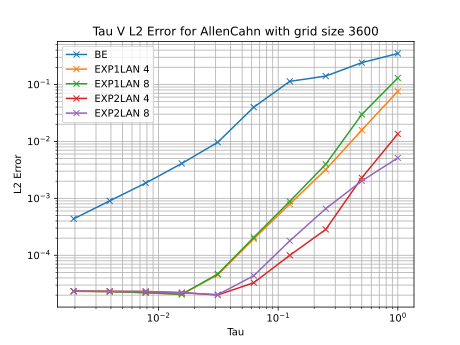
\includegraphics[width=1\textwidth]{Graphs/AllenCahn/Tau V L2 Error for AllenCahn with grid size 3600.png} % Change filename to your image
        \caption{$\tau$ vs $L_2$ with grid size 3600}
        \label{fig:ACtauE1024}
    \end{minipage}\hfill
\end{figure}

We observe convergence in both expoential methods for both krylov sizes.
These methods significantly outperform the backwards Euler method, simillar to the traveling wave Allen Cahn problem given above.
For this problem a relatively shallow subspace has been used compaired to above and appears to be sufficient.

Below as before we present the number of calls to the operator against the error.
\begin{figure}[H]
    \centering
    \begin{minipage}{0.49\textwidth}
        \includegraphics[width=1\textwidth]{example-image-a} % Change filename to your image
        \caption{$\tau$ vs $L_2$ with grid size 1024}
        \label{fig:plot1}
    \end{minipage}\hfill
    \centering
    \begin{minipage}{0.49\textwidth}
        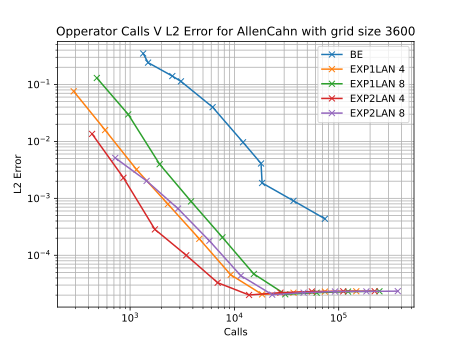
\includegraphics[width=1\textwidth]{Graphs/AllenCahn/Operator Calls V Error for AllenCahn with grid size 3600.png} % Change filename to your image
        \caption{$\tau$ vs $L_2$ with grid size 2048}
        \label{fig:plot2}
    \end{minipage}\hfill
\end{figure}
For both methods we see that to achive a lower error requires more calls to the operator.
We see that in terms of performance the backwards Euler method performs significantly worse in comparison to both of the expoential methods.

Here we present the experimental orders of convergence.

\begin{table}[H]
    \centering
    \begin{tabular}{| c | c | c |}
    \hline
    BE & EXP1LAN 8 & EXP2LAN 8 \\
    \hline
    0.5336772856567727 & 2.124425468811078    & 1.3416905476319223 \\
    0.7835756762460372 & 2.905742997002231    & 1.6172444544625373 \\
    0.3087677833100485 & 2.1667343028183392   & 1.8766417619133886 \\
    1.504631886802277  & 2.0994616006682154   & 2.034301870712038 \\
    2.0486348034911237 & 2.13577903687606     & 1.1061518243743675 \\
    1.237052619854426  & 1.184386408121027    & -0.11660694297267732 \\
    1.1376542802507796 & -0.09373274955254216 & -0.06785678855256895 \\
    1.0396362359013922 & -0.06516215516412459 & -0.005698148120031917 \\
    1.0482179972577244 & -0.01797864948877803 & -0.01442779444997218 \\
    \hline
    \end{tabular}
    \caption{Reduced Data Table}
    \label{tab:reduced_data}
\end{table}

Again we observe first order convergence for the backwards Euler methods and second order convergence for the two exponential integrator methods.
